\documentclass[10pt]{IEEEtran}
\usepackage{lipsum}
\usepackage{graphicx}
\usepackage{amsmath}
\usepackage{listings}
\usepackage[]{algorithm2e}
\RestyleAlgo{boxed}
\lstset{language=C++}
\begin{document}
\title{Building a SLAM System for an Autonomous Surface Vehicle}
\author{Daniel~Snyder
\thanks{Thank you to Dr. Ryan Eustice for being my Advisor on this project
}}
\maketitle
\begin{abstract}
One of the fundamental problems in autonomous mobile robotics is that of simultaneous
localization and mapping (SLAM).  Solving SLAM involves the robot simultaneously
determining both its position in the environment (localization) and what its environment
is (mapping), which are problems dependent on each other.  This problem is essential to
many of the other problems present in autonomous mobile robotics.  If a robot does not
know its location and its environment it cannot complete tasks such as navigation.  
 
There exists many approaches to solving the SLAM problem, and each approach has
its own drawbacks and advantages.  The goal of this project is to implement and
compare multiple solution methods to determine their advantages within a specific
domain.  The solutions will be evaluated in the context of an aquatic autonomous surface
vehicle (boat) designed and built by the UM::Autonomy student team at the University
of Michigan for participation in the International Roboboat competition hosted by
the Association for Unmanned Vehicle Systems International (AUVSI).   
  
In particular a graph-based solution using the incremental smoothing and mapping
(iSAM) method, and a solution using an occupancy grid for mapping along with a 
monte carlo localization using a particle filter for localization (GM-MCL) will be implemented and compared
to the Extended Kalmann Filter (EKF) based SLAM that has been implemented by previous
UM::Autonomy team members.  Their performance will be evaluated based not only on
actual task performance, but also on the ease of understanding and maintainability
of the system over time.  The focus on ease of understanding and maintainability
arises from past challenges the current EKF SLAM implementation has presented to the team. 
\end{abstract}

\section{Overview of the SLAM Problem}
SLAM is a problem fundamental to autonomous robotics.  In order for a robot to accurately
traverse and interact with its environment, it needs to know what the environment is 
(mapping) and where it is in the environment (localization).  While for some applications it
is possible to generate a map in advance, for many applications, it is necessary to perform 
both localization and mapping at the same time.  The difficulty lies in that in order to 
accurately map, the robot must know its location, and that in order to find its location, the
robot must have some form of a map.  SLAM techniques attempt to solve this problem through 
various methods.  This paper will look at two such methods, and analyze their applicability
to an autonomous surface vehicle (ASV) built by a student team at the University of Michigan.

\section{Research Goals}
The primary goal of this research is to create a SLAM system that 
UM::Autonomy can use for years to come.  Inherent within this goal are a few criteria that
are required for the goal to be achieved. These criteria fall into three categories:
performance, useability, and maintainability.

\subsection{Performance}
The first set of criteria that this research must satisfy is that of performance
requirements.  The end product must work reasonably well in a multitude of environments and
must fit within the computing capabilities of the autonomous surface vehicle (ASV).
The end product
should be able to perform online SLAM, approximating a solution to the SLAM problem in 
real time, while allowing the team to run other code simultaneously.

\subsection{Useability}
Beyond performance, the SLAM system produced must be easy to use.  A majority of the 
people using the system will not have much knowledge of how the SLAM problem is solved,
so its use cannot require multiple steps or indepth knowledge of the solution method.

\subsection{Maintainability}
The maintainability of the system is most crucial to assuring its prolonged usage.
In the past, the team has neglected the SLAM system due to its complexity, and over time
this has caused the system to degrade in quality.  Large consideration will therefore 
be put into code quality and design.  The code should be designed with maintainability in
mind to prevent degredation over time.

\section{Document Purpose}
This document is meant to serve two purposes.  The first purpose is to provide a 
technical explaination of the research conducted on the SLAM problem.  The second
purpose is to serve as a technical reference for UM::Autonomy for understanding and extending
the SLAM solution that is presented.

\section{Capabilities of the Autonomous Surface Vehicle}
As the system was designed for use with the Autonomouse Surface Vehicle (ASV) that is
built by UM::Autonomy, the solution approaches are heavily dependant on the capabilities of
the platform.  The ASV is equipped with a Global Positioning System (GPS), a fiber optic 
gyroscope (FOG) and a panning Lidar with a 270 degree field of view.  Together, these sensors
allow the ASV to obtain an approximate global pose and to survey the local area.

Beyond the current sensors on the ASV, the team is also planning to add an inertial 
measurement unit (IMU) and a compass.  In order to meet maintainability requirements, it
is important that these sensors are also considered when performing the research.

\section{Solution approaches}

\subsection{Incremental Smoothing and Mapping}
iSAM draws on the work of Kaess et al.\cite{iSAM}.  iSAM is a feature
based SLAM, meaning that it represents the world using the features the robot observes, using
the
features to build a map and localize itself within the map.  This means that iSAM is heavily 
dependent on having proper feature detection and matching.

\begin{figure}
	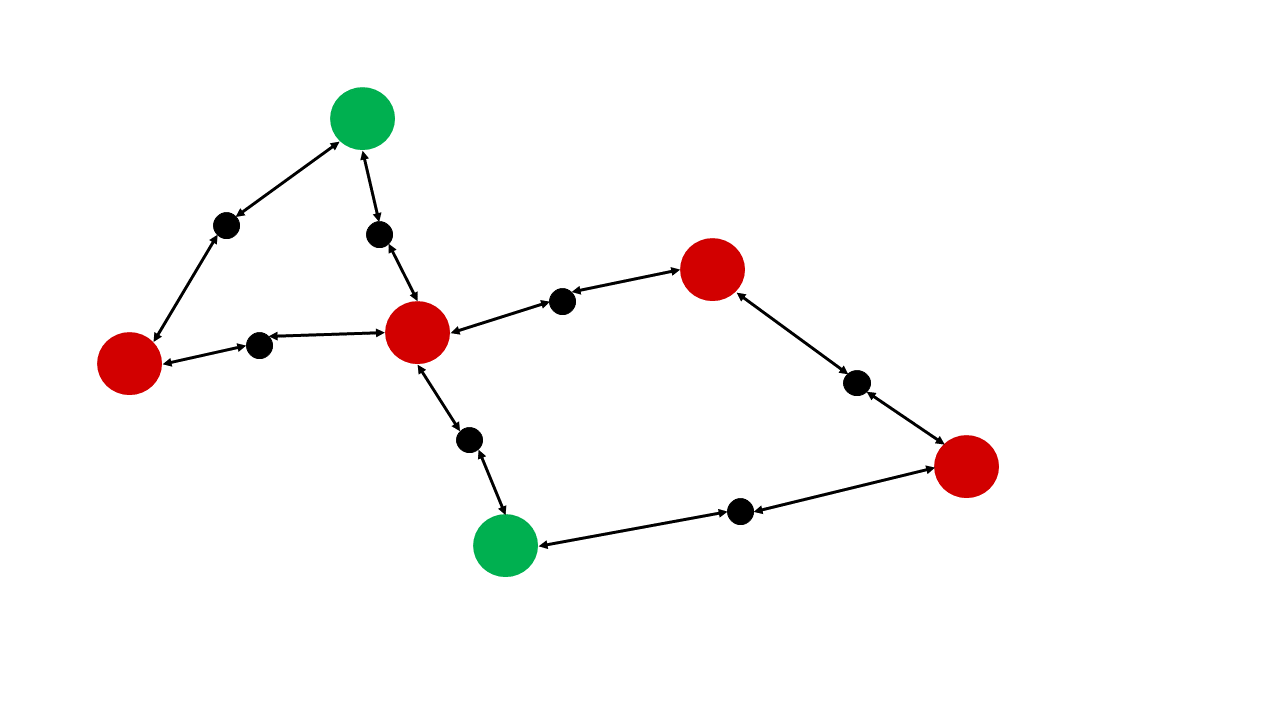
\includegraphics[width=\columnwidth]{Figures/isamGraph}
	\caption{Example graph structure for an iSAM based solution}
	\label{fig:iSAMGraph}
\end{figure}

iSAM represents the world using a graph structure.  The
graph contains two types of nodes; poses and factors.  Poses represent the position of an
feature or the position of the robot.  Factors are used to connect one pose to another, and
represent the relationship between the two poses and the probabilities associated with those
relationships.  An example graph structure can be seen in Figure \ref{fig:iSAMGraph} where the red circles
are the poses of the robot as it goes through the environment, the green circles
are the landmarks that are observed as the robot traverses the map, and the black circles
are the factor nodes representing the observations and information that connects two pose 
nodes.

After creating this graph, iSAM attempts to optimize it, combining multiple observations
into one to reduce the size of the graph while preserving all the information. By performing
these optimizations, future updates are easier to perform, making iSAM much faster than
other state of the art methods.

For this approach, the Perceptual Robotics Laboratory's iSAM library was used as a back-end 
with a custom front-end built around it.  The back-end was previously verified and is capable
of anything the ASV would need, meaning that the team would not have to do much 
to maintain this approach.  However, the front end is quite complex as the graph structure
can have multiple valid representations, that all perform differently.   In the end, the
team was unable to create a fully working iSAM-based system due to issues with feature
detection and difficulties with the front-end implementation.

\subsection{Occupancy Grid based Mapping and Monte-Carlo Localization}
In contrast to iSAM, the GM-MCL method is not a feature based SLAM method.  Rather than representing
the map and the robot's location in it as a graph, the map is represented
as a grid, where each cell contains a probability that the area of the world it represents 
contains some object.  In this way, GM-MCL is based only on the probability that a given area
of the world contains an  object, rather than the nature of an object.

This method is derived from slides made by Dr. Kuipers for EECS 467 at the University of
Michigan with Monte Carlo Localization being based on \cite{MCL}.  The method works by first generating a set of particles all located at the origin
of a map where all cells have an equal probability of either containing (being full) or
not containing (being empty) an object.  The first map is then generated from a
lidar scan and set as the current map.  For every subsequent set of lidar data that comes in,
Monte-Carlo Localization is first performed, and a new most likely location is selected.
Then the map is updated based on the lidar data at the new location, generating an
updated map.  This process is then repeated until termination.  This algorithm
can be seen in graphical form in Figure \ref{fig:SlamAlg}. 

The primary benefits of this method derive from is its lack of reliance
on landmark detection and classification.  Due to the nature of the student team, it is 
beneficial to limit dependencies between the various systems.  Previously, the team had
relied on SLAM to do the classification and data association for landmarks, which 
expanded the scope of the SLAM system and created issues with maintaining the old EKF
implementation
By separating out landmark related compuational tasks, the 
algorithm is less dependent on landmark detectors, making it easier to maintain and debug.

Another benefit of GM-MCL is its simplicity and understandability.  Compared to algorithms
such as EKF and iSAM, GM-MCL is relatively simple and requires much less understanding in 
order to develop and maintain.  Past experiences explaining GM-MCL to teammates have shown
that most of the algorithm can be explained without any reliance on the mathematics and 
probability theory behind the method.  In the end, this leads to a method that fits the
criteria for maintainability by being easy to understand and maintain, without extensive prior knowledge.

\begin{figure}
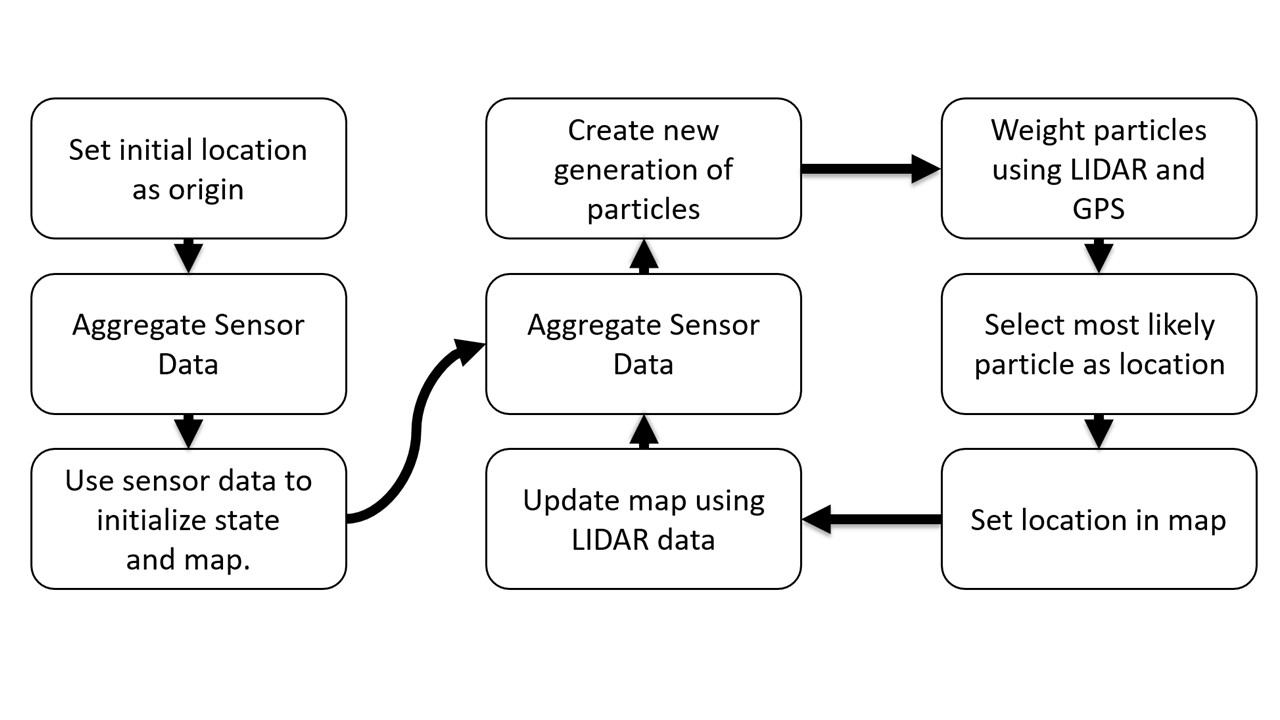
\includegraphics[width=\columnwidth]{Figures/slamAlg}
\caption{Algoritm used in GM-MCL method.  Includes initialization, localization, and mapping steps}
\label{fig:SlamAlg}
\end{figure}

\section{Analysis of Approaches}
In order to accurately analyze the two approaches in the context of the ASV and a student
team, criteria for analysis must be established.  For performance, useability, and 
maintainability, various criteria were established by which the methods will be compared.
These criteria can be seen in Figure \ref{fig:AnalysisCriteria}.

\begin{figure}
\begin{tabular} { r | l }
	Category & Criteria \\
	\hline Performance & Computational Resources Required \\
	Performance & Quality of Map Generated \\
	Useability & Reliance on Knowledge of SLAM Problem \\
	Maintainable & Number of External Dependencies \\
	Maintainable & Amount of Knowledge Required to Maintain \\
	Maintainable & Difficulty of Implementation
\end{tabular}
\caption{Table representing criteria for comparing the two methods}
\label{fig:AnalysisCriteria}
\end{figure}

\subsection{Performance Criteria Analysis}
In the end, the GM-MCL approach was found perform better in these criteria than iSAM did.
When looking at the computational resources required, in contrast to the claims made by 
Kaess et al. \cite{iSAM_website} that iSAM is the incredibly efficient and fast, 
the iSAM implementation requires more computing resources than the GM-MCL approach.  The 
iSAM backend that was used utilized multiple threads and
 was a separate program from the front end, and is capable of causing network congestion
due to the reliance on LCM for communication between the front end and back end.
In contrast, the GM-MCL implementation is single threaded
and due to the configurable number of particles used by Monte Carlo Localization, the 
computational resources required can be decreased or increased based on availaiblity.  It
is possible that for large data sets, iSAM requires less computational resources, but in
the context of the ASV, the amount of computational resources used by iSAM were much greater 
than those used by GM-MCL.  This is
possibly due to the generality of the iSAM approaches back-end,
where as the GM-MCL approach is tailored
to the specific needs of the ASV.

When comparing the maps the two methods generated, issues arose.  The iSAM implementation was
never capable of generating a full map, so the quality of the maps are not comparable.  
However, since iSAM is state of the art, it will most likely generate a more accurate map.
Additionally, due to the nature of using an occupancy grid for large
maps with sparse features, as is the case for the ASV, it is likely that a feature based
approach will require less memory to maintain and will be easier to share between processes. 
If both approaches could be accurately compared in this area, it is theorized that iSAM would
perform better than GM-MCL.

\subsection{Useability Criteria Analysis}
In terms of useability, GM-MCL is easier to use than the iSAM implementation.  The GM-MCL
implementation builds a single executable, whereas the iSAM implementation generates three
executables, one for the back-end, one for the front-end, and a third for visualization 
of the map.  Due to the larger amount of executables that need to be run with
the iSAM implementation, it requies more overhead knowledge as it is possible, and has happened,
that one executable is forgotten and that is not desireable.  Additionally, the iSAM solution
is much more reliant on prior knowledge of the SLAM problem.  The method uses more math and 
requires a deeper understanding of probability thoery to understand how it works, and what is
going wrong.  Due to this barrier in understanding, GM-MCL appears to be a much more useable
than the iSAM implementation.

\subsection{Maintainability Criteria Analysis}
In implementing the iSAM method, it became clear that it was a less maintainable solution
than the GM-MCL solution.  The iSAM solution was itself an external dependency and had a few 
other external dependencies.  Due to the complexity of the mathematics surrounding iSAM, it
was more difficult to develop and there were small differences between an efficient
implementation and an inefficient implementation.  For the same reason it also became
apparent that maintaining the iSAM implementation would be very difficult as it could easily
decay in performance.

\subsection{Conclusion}
The results of the comparison can be seen in Figure \ref{fig:CriteriaComp}.  The GM-MCL
method was found early on to be much more favorable to the iSAM solution.  The 
maintainability and useability 
problems that arose in the iSAM solution outweighed the potentially better performance.
\begin{figure*}
\begin{tabular} { r | l }
	Criteria & Results \\
	\hline Computational Resources Required & GM-MCL Requires less computational resources\\ 
	Quality of Map Generated &  iSAM is most likely capable of generating the better map\\
	Reliance on Knowledge of SLAM Problem &   GM-MCL requires minimal background knowledge of the SLAM problem\\
	Number of External Dependencies  &  GM-MCL does not rely on any feature detectors, and is more self contained\\
	Amount of Knowledge Required to Maintain &  GM-MCL requires less mathematical and robotics knowledge to maintain\\
	Difficulty of Implementation &  ISAM is much more difficult to implement
\end{tabular}
\caption{Table showing the results of the criteria analysis}
\label{fig:CriteriaComp}
\end{figure*}

\section{SLAM Related Utilities}
In order to create a SLAM program that is performant, useable, and maintainable, a few 
SLAM related utilities were created during development.  These utilities are a 3D Point Cloud
that is generated from a panning LIDAR and a simulated compass.

\subsection{3D Point Cloud Generation}\label{pointcloud}
One feature of the robotic boat is a panning LIDAR that allows for generation of a three 
dimensional point cloud.  This point cloud allows for detection of objects floating on the
water's surface in addition to objects that are raised off the water's surface. 
For this research, a method for transforming the scans generated by the point cloud was 
developed.  

The method uses quaterions to take a lidar return from \(<r, \phi, \theta>\) to 
\(x,y,z\) which represented the forward, right and down directions respectively.  
This transformation can be seen in equations \ref{eq:Qx}, \ref{eq:Qy}, and \ref{eq:Qz}.

\begin{align}
	\label{eq:Qx}
	x = r\cos(\theta)\cos(\phi) + d \sin(\theta) \\
	\label{eq:Qy}
	y = -r \sin(\theta) \\
	\label{eq:Qz}
	z = r \cos(\phi)\sin(\theta) - d \cos(\theta) 
\end{align}

A key feature of the point cloud generator is its representation of scans that did not 
return any information (the scan did not encounter an object within its range).  In order
to accurately map the empty space that these scans represent, their directional information
must still be passed to the mapping algorithm.  This information is represented by giving
each lidar return an associated 8-bit integer that represents whether or not the lidar
return used to generate the point encountered an object.  If no object is encountered,
the lidar point is given a default range that it traveled, and is marked as not having 
encountered an object.  Doing so allows the mapping algorithm to accurately categorize 
large amounts of empty space as empty.

\subsection{Simulated Compass}
A challenge that the team has faced in the past few years is the lack of a compass.  
The boat uses the NED (North East Down) coordinate system, so if north cannot be found, 
the coordinate system may be set incorrectly.  In the past the team has solved this by
manually position the ASV to be facing north when starting the software,
a process that is subject to human error. To remedy this until the team adds a compass to the ASV,
a method was developed to simulate a compass.  The fake compass listens to changes in GPS
data, then from the change in GPS data, recalculates the offset needed to 
orient the coordinate system properly.  After the ASV has moved a certain amount
of distance from the origin, the map is reset, the coordinate system is reoriented,
and the SLAM process is restarted with a new map.

When testing the simulated compass, the tests showed mostly proper results, with the 
coordinate system being correctly reoriented in most logs.  However, in sensor logs where 
the ASV remained still for long periods of time, or was pointed in a direction close to 
north, meaning that the coordinate system did not need to be reoriented, the simulated
compass did not work properly.  To account for this,
there is an option to turn off the simulated
compass for logs and situations where it is not necessary.  More 
investigation as to the source of this error is an area for further research.

\section{In depth explaination of occupancy grid and particle filter approach}
The purpose of this section is to explain in depth the various aspects of the GM-MCL
solution method.  This section will discuss the specific adjustments made to the generic
approach to better fit the ASV's application.

\subsection{Initialization}
There are two different phases of initialization.  The first phase is the compass phase.
In this phase, the coordinate system is either initialized or reoriented to be a north, east
down (NED) coordinate frame.  This process is either performed using a compass, or
a simulated compass, as described previously.  After the coordinate frame is correctly
oriented, the next phase is initializing the map.  In this phase, the ASV is assumed to not
move and a configurable number of point clouds are received and the map is generated to
provide an initial starting point from which to build future maps.  After initialization,
the system waits for more point cloud data.  Every time it receives point cloud data, 
it first localizes itself, and then updates the map.


\subsection{Creating Particles to be Filtered}
In prior implementations particles, for the current generation were created from sampling from
the previous generation of particles, and applying a change in location based on odometry 
data plus some error.  For the ASV however, there is currently no sense of odometry that 
can be used to link the previous generation to the current generation.  Additionally, the 
team will be adding an IMU to the ASV, giving a sense of odometry.  To allow for easy 
integration of the IMU, two types of particles, distinguished by the method used to create
them, were developed; generational particles and non-generational particles.

After generating the set of particles from the two methods, the particles only contain X and
Y coordinates.  To get the theta for each particle, each particle samples from a gaussian
distribution centered at the last FOG measurement.  This generates a set of possible yaws
for the ASV.  These particles are then weighted based on lidar data.

\subsubsection{Generational Particles}
Generational particles are particles that are created by sampling the previous generation of
particles, and predicting them forward based on odometry data. Currently this is done using
the change in GPS data to predict a particle forward.  However, since GPS gives a sense of 
global location rather than change in local location, it is not an ideal source of odometry
data.  It is recommended that an IMU is used to generate the odometry data, even though that
is outside of the ASV's current capabilities.  Despite the lack of an IMU, this method was
developed to ease extension of the code.  Having the framework in place to generate 
generational particles allows for easy IMU integration, preventing a potential source of 
code quality degredation.

\subsubsection{Non-Generational Particles}
Non-generational particles are particles created from sampling a two dimensional gaussian
distribution whose mean is the last received GPS coordinate.  This creates a set of particles
that are independant of the previous generation.  The benefits of this approach lie in its 
ability to correct within symmetric environments.  Since GPS is a global position, it is 
more robust to errors created by a misprediction in locally symmetric maps.  
By using non-generational particles, the progam assures that there always exists some 
particles in the area closest to the global location of the ASV. %reword this

%This may not be the correct place for this
Another benefit to the non-generational approach is that it allows for GPS only localization.
By using only non-generational particles and weighting based only on GPS, the pose will 
be determined based only on the GPS location.

\subsection{Weighting the particles}
After generating the particles for the current particle filter, it is necessary to determine
which particle is the most likely position based on sensor data.  This section describes 
the mechanisms by which particles weighted. Overall, the general priciple is that each sensor
assigns a weight to a particle that is bounded within a certain range.  This weight is then
multiplied by a configurable coefficient.  The coefficients were made to be configurable 
to allow the addition of new sensors and easy tuning and maintenance for the coefficients.
This section will describe the various methods each sensor uses to generate weights.

\subsubsection{Point Cloud Weight Generation}
The weight of a particle based on point cloud data is determined by checking how well the
point cloud matches the map from each particle's pose.  Each point in the point cloud is 
rotated into global coordinates based on the particle's pose.  Then, if the point was marked
as hitting an object, the end point of the
particle is checked to see if there is an object at that location.  If the end cell 
contains an object, a hit occurred, the likelihood of the particle is increased.  If the end
cell does not contain an object, a miss occurred, the likelihood is heavily decremented, due to the accuracy
of the lidar sensor.

This process is repeated for each particle to get a set of weights based on point cloud data.
These weights are then rescaled to be in the range \([0,1]\) 
to make the point cloud based weights easily comparable to the weights 
generated by other sensors.

Weight generation based on point cloud data is done using a hit or miss approach for two
reasons.  The first reason is efficiency, there is a large amount of data in each point cloud
and doing hit or miss makes processing this data faster than approaches such as stepping
from the ASV's location to the lidar's end point, and allows the localization to run in real
time. Additionally, due to representing a three dimension word in two dimensions, it is 
possible for some lidar scans to be at a different height than others, which could cause
erroneous assumptions that a lidar return missed an object when in actually went over
the object.  The hit or miss approach is also applicable here due to the accuracy
of the lidar the 
ASV uses.  The lidar has a standard deviation of 30 millimeters, which means that checking
squares close to the end point would yield minimal additional information due to the square
size being 0.5 meters.

\subsubsection{GPS Based Weight Generation}
The weight of a particle based on GPS is determined by taking the location of each particle
and finding probability of that location based on the gaussian distribution that is used to 
create the non-generational particles.  The weighting based on GPS data has the benefit of 
increasing the likelihood that the global position is close enough to the last measured GPS 
point.  By tuning the coefficient for the GPS weights, the most likely particle can be biased
to be farther from or closer to the last GPS point.

\subsubsection{FOG Based Weight Generation}
The weight of a particle based on FOG measurements is determined by finding the probability
of a particle's theta based on the gaussian distribution used to create the theta for each of
the particles.  By decreasing the coefficient of theta, the correct rotation of the lidar
data is more likely to be selected as the actual pose, even if the map is shifted.  
By increasing the FOG coefficient, the FOG data is believed more, which can be used to dealt 
with drift in the FOG data overtime.

\subsection{Filling the Map}
After selecting the particle with the highest weight as the most likely location, the system
fills in the map using the same point cloud that was used to localize the ASV.
The mapping process takes in the location of the ASV, and the most recent point
cloud generated by the three dimension point cloud generator discussed in Section
\ref{pointcloud} and uses the three dimensional coordinates that it returns to fill in the 
map.  For each point generated by the point cloud, the mapping algorithm first transforms
it from local coordinates to global coordinates.  Then, the algorithm steps along the line
connecting the boats current location to the location at which the lidar returned.  If the
current grid cell the algorithm steps into is not where the lidar encountered an object,
it is marked as empty and the probability that it contains an object is decreased.  When
the grid cell that the lidar point returned from is reached, the probability
that an object resides in that area of the map is increased.  However, if the lidar return
did not encounter an object, as determined by the associated 8-bit integer, the ending grid
cell is marked as empty.  This process is repeated for all of the points in the point cloud,
and is summarized in Algorithm \ref{mapalg}.

\begin{algorithm}
	\label{mapalg}
	\KwData{PointCloud pc, GridMap map, ASV\_Pose pose}
	\KwResult{Updates the map based on the information in point cloud}
	\For{3DPoint p in pc}
	{
		RotateIntoGlobalCoordintes(p, pose)\;
		ASV\_Pose curr\_pose = pose\;
		//gets the cell number that a 3D point resides in\\
		int end\_cell = map.getCellNumber(p)\;
		int curr\_cell = map.getCellNumber(curr\_pose)\;
		\While{curr\_cell != end\_cell}
		{
			map.updateAsEmpty(curr\_cell)\; 
			//step curr\_pose along line connecting pose to p \\
			stepForward(curr\_pose, pose, p)\;
			curr\_cell = map.getCellNumber(curr\_pose)\;
		}
		\eIf{p.hitObject == 1}
		{
			map.updateAsFull(end\_cell)\;
		}{
			map.updateAsEmpty(end\_cell)\;
		}
	}

	\caption{Algorithm used to update the map based on the point cloud and current location}
\end{algorithm}

\section{Special Considerations}
The largest challenge encountered in the course of research was the nature of the ASV.  
The ASV has limited computational capabilities, and has limited sensing capabilities.  
To account for these shortcomings, considerations had to be made as to how to address the
problems faced by the ASV.  This section details some of the special considerations made
for the ASV.

\subsection{Representing the 3D world in 2D}
For simplicity, maintainability, and efficiency, it is desireable to represent the world in
two dimensions (x,y) rather than three (x,y,z).  By representing the world as a
bird's eye view, the problem of objects having a limited height occurs.
For a top down view, it is desirable to mark a grid cell as full if at any height,
an object exists in that cell.  However, the panning lidar does not see the entire z axis 
of the world, leading to some gaps in the data about the three dimensional
world.  To remedy this, a few steps were taken.  The first step is to limit the range
of lidar data that is being processed.  By limiting the lidar data to only the data that
represents all parts of the z axis that are desired, it can be assured that no objects are
removed from the map due to a lack of information at a given height.  The second
step taken to better represent the world in two dimensions occurs when filling in the map.
When filling in the map, if a point cloud ever sees a grid cell as full, it will be marked
as full for that entire mapping process, no matter how many other lidar returns would
mark it as empty.  This prevents an object located on the
water's surface from being removed from the map by lidar scans that pass over it.  By 
combining these two techniques the three dimensional world is better able to be
represented using a two dimensional grid.

\begin{figure}
	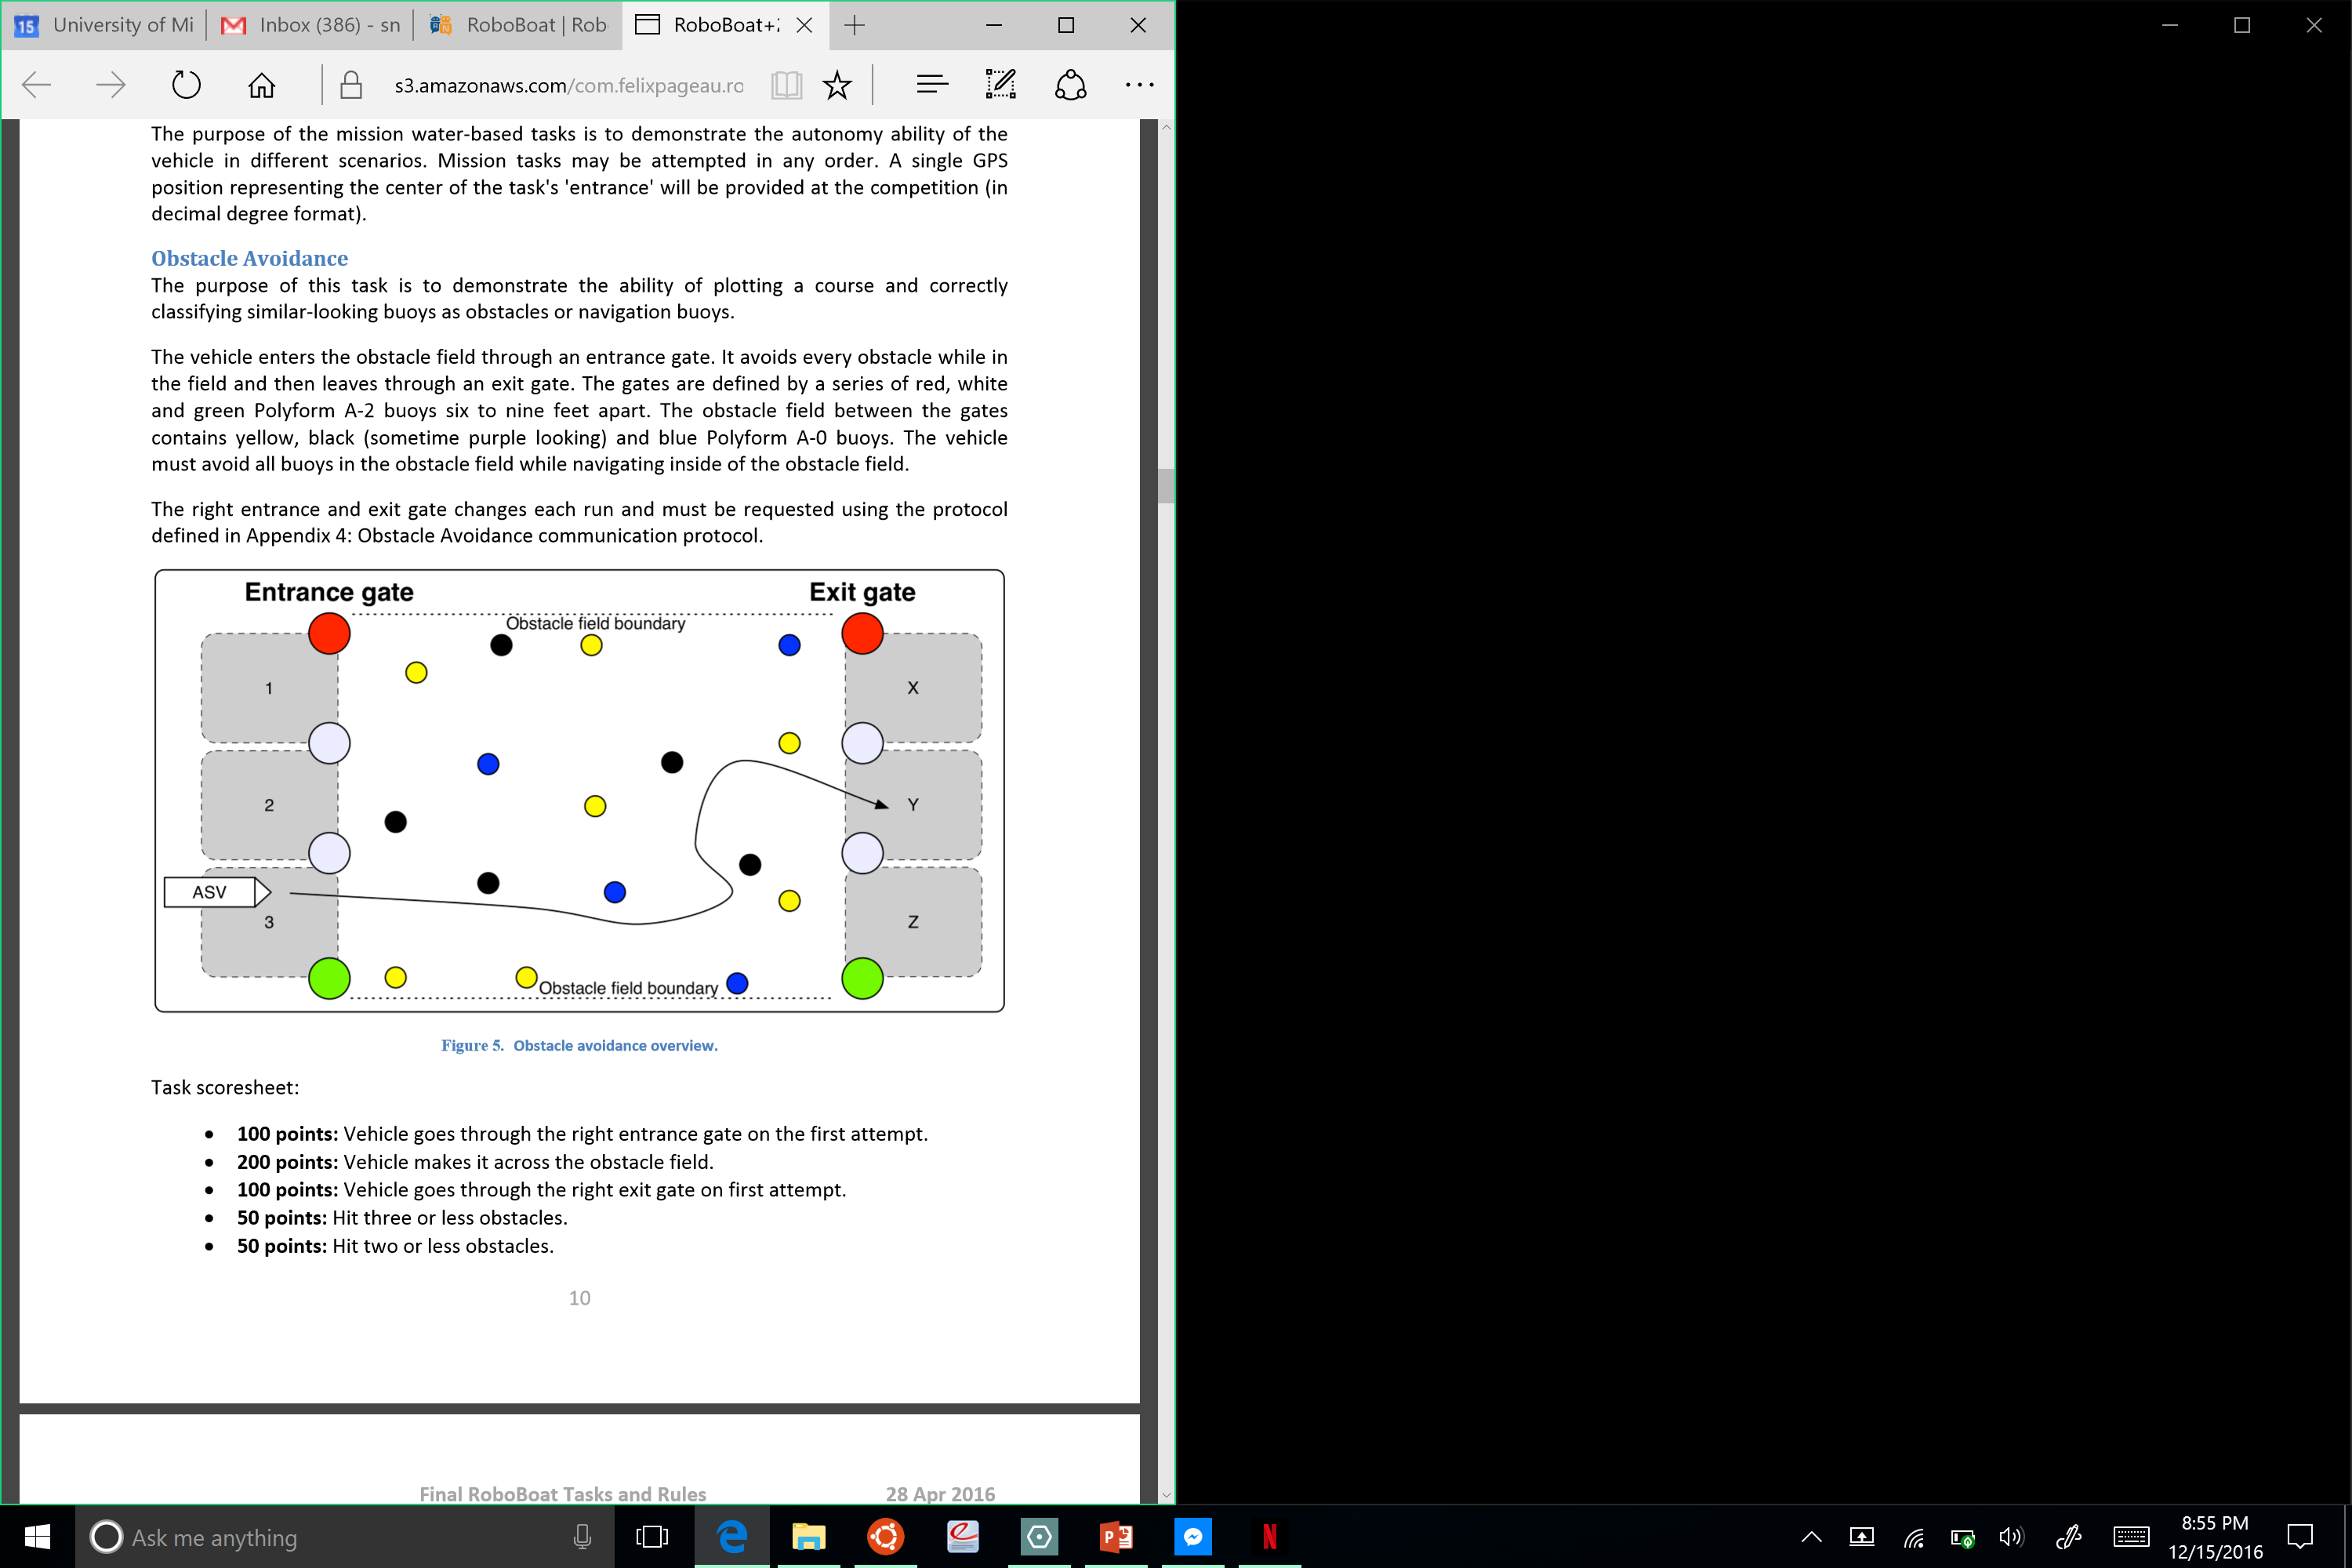
\includegraphics[trim={5cm, 25cm, 55cm, 25cm}, clip, width=\columnwidth]{Figures/roboboatObs}
	\caption{Example buoy course map}
	\label{fig:RoboBoatObs}
\end{figure}

\section{Results}
This section looks into the results of the research.  The overall results will be discussed,
and then the effects of changing various factors within the SLAM algorithm will be 
analyzed.  The goal of this is to provide insight into how the algorithm reacts to changes
and how those changes can be used to adapt and tune the SLAM system to better suit the 
needs of the ASV.  

Each test is conducted by first changing one variable and comparing it to the baseline.
The baseline performance is the combination of constants that have been shown to perform
well in a variety of circumstances.  Testing will be performed on a past sensor log that
contains actual data the ASV received while at the RoboBoat Competition.

The log is the sensor data that was received as the ASV moved through the obstacle course
challenge.  This map 
should resemble the example obstacle course in the RoboBoat Final Rules, seen in 
Figure \ref{fig:RoboBoatObs}, with some movement
in the obstacles.  The obstacles in question are buoys that reside on the water's surface.
This log tests the performance of the system when there are no long straight surfaces such
as walls to localize and map on.


\subsection{Baseline Performance}
The baseline is the set of constants that performed the best in a multitude of environments.
The constants file used for the baseline can be found in Appendix A.

\begin{figure}[h]
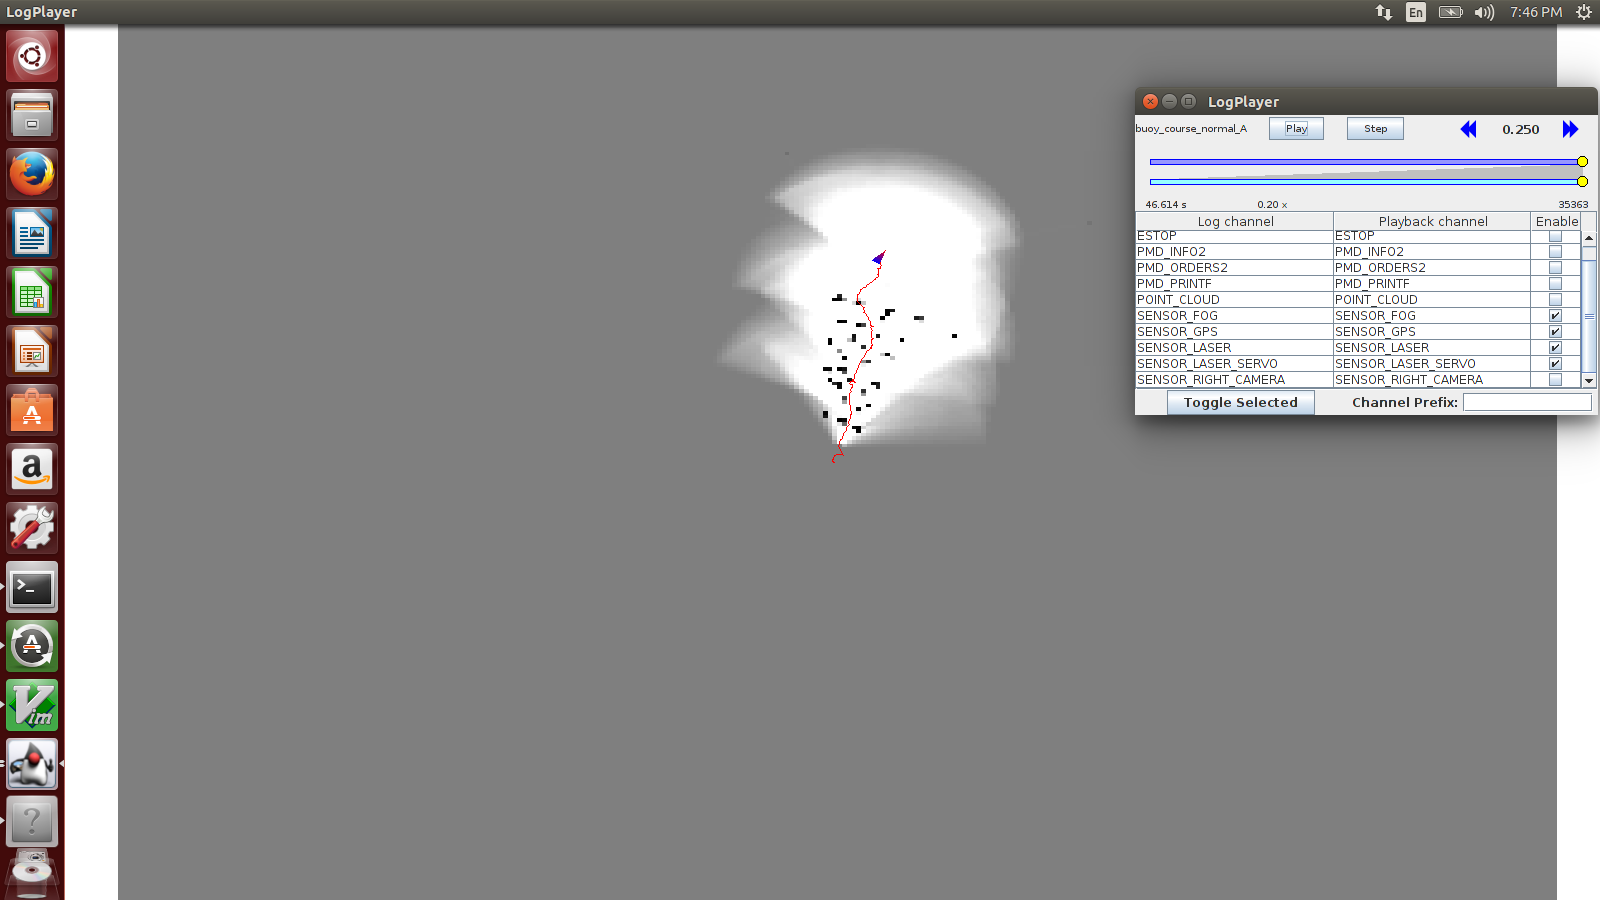
\includegraphics[trim={25cm 15cm 20cm 7cm}, clip, width=0.9\columnwidth]{Figures/baseline1}
\caption{The baseline image to which all others are being compared}
\label{fig:Baseline}
\end{figure}

\begin{figure*}[!ht]
\centering
		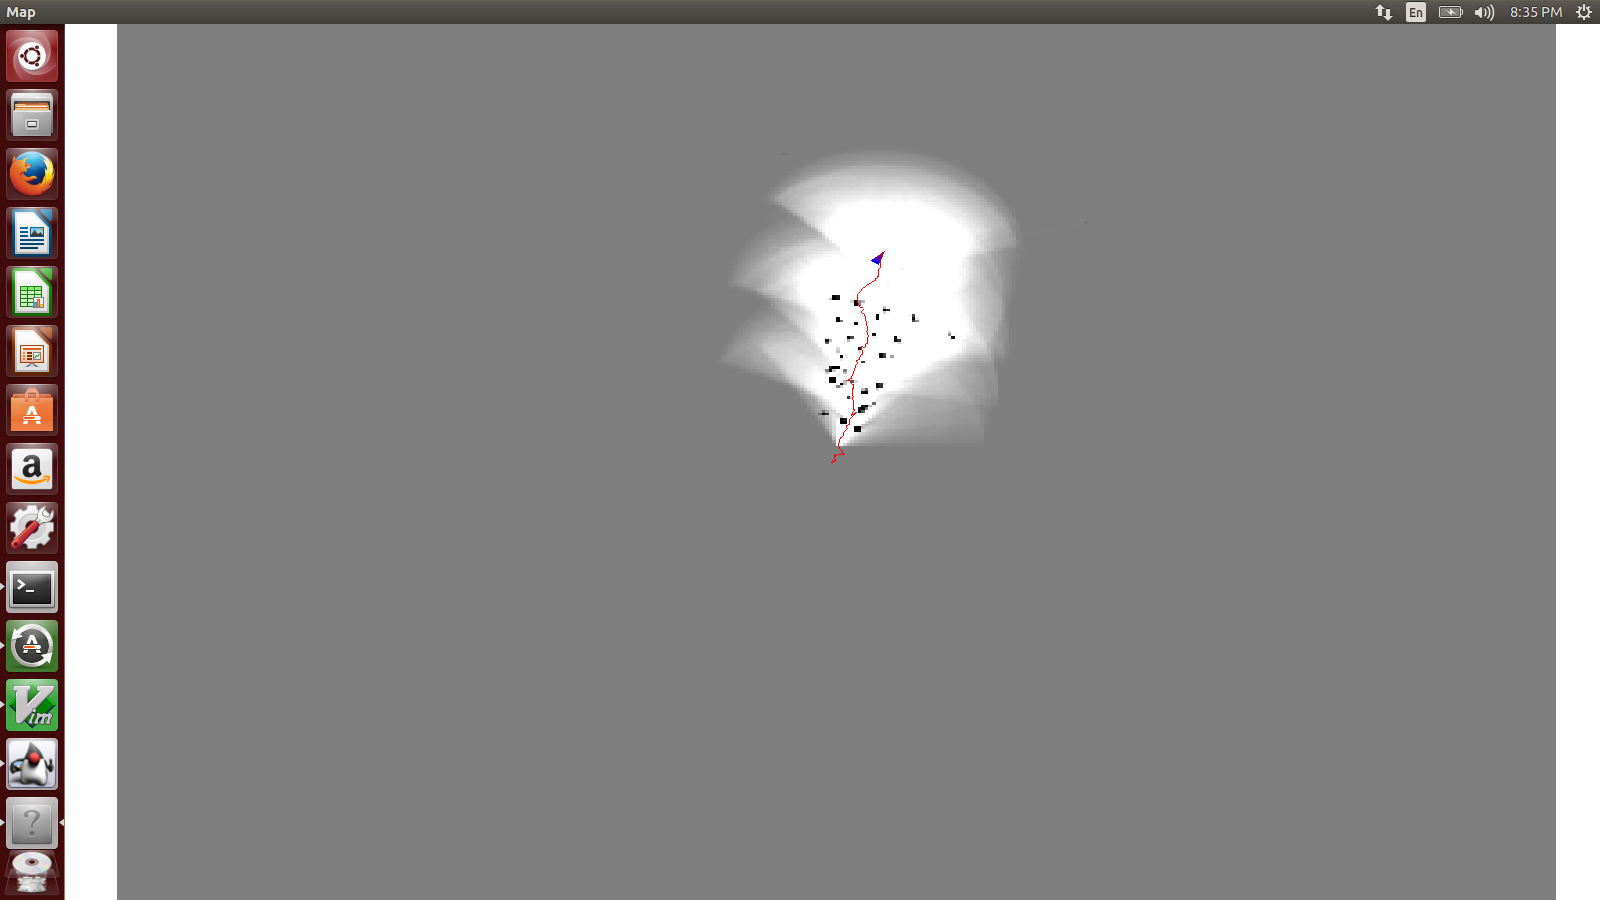
\includegraphics[trim={25cm 15cm 20cm 7cm}, clip, width=0.3\textwidth]{Figures/smallGrid}
		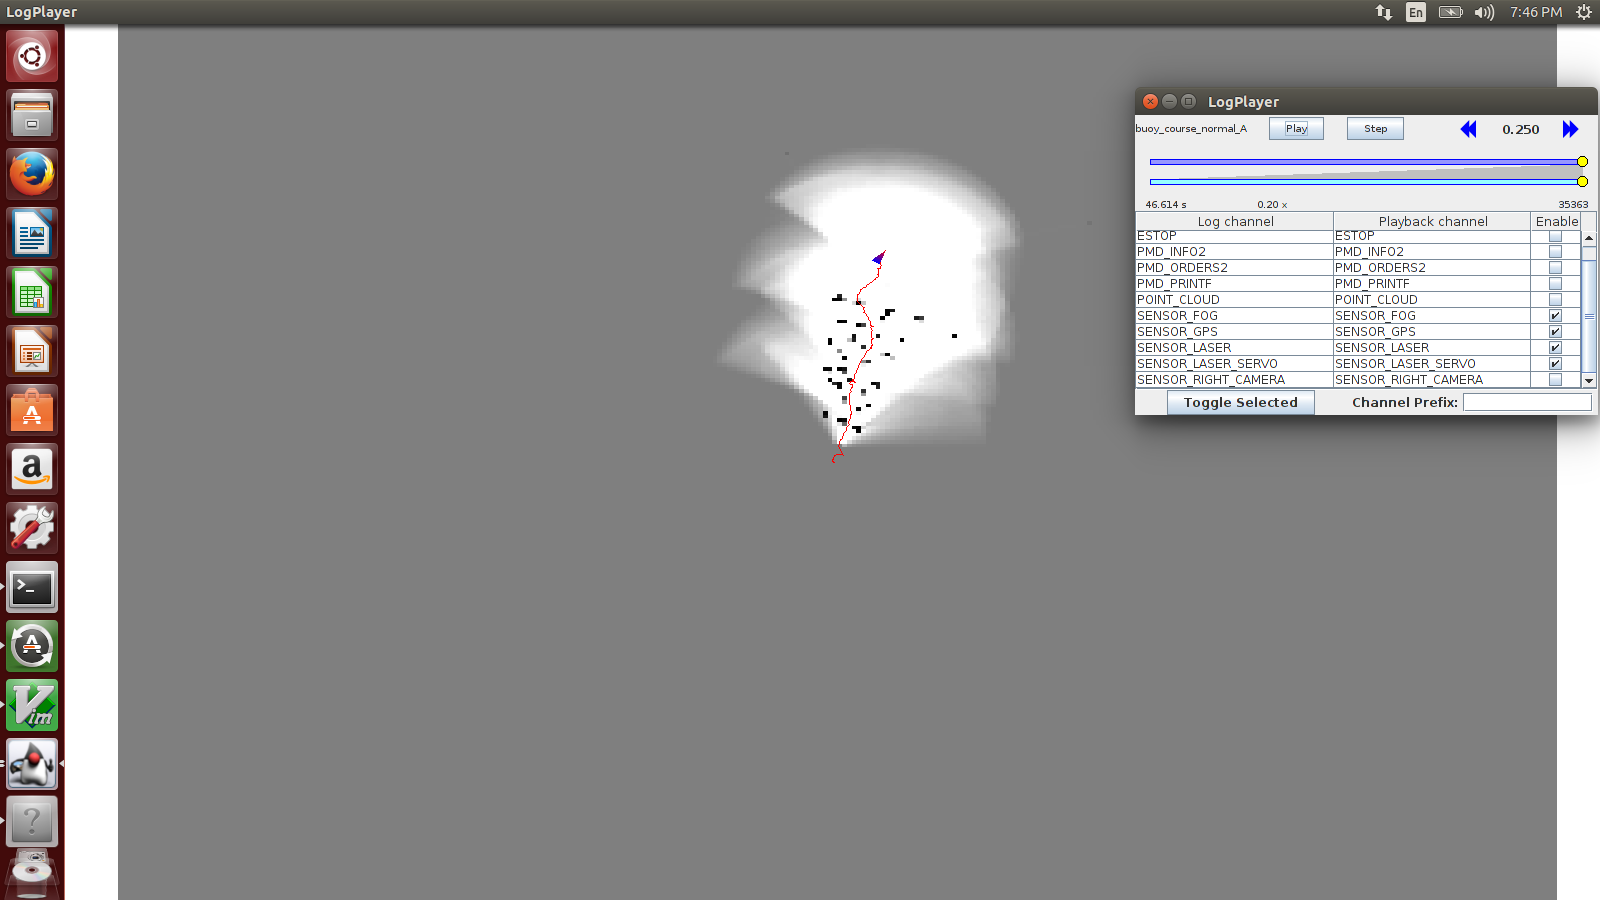
\includegraphics[trim={25cm 15cm 20cm 7cm}, clip, width=0.3\textwidth]{Figures/baseline1}
		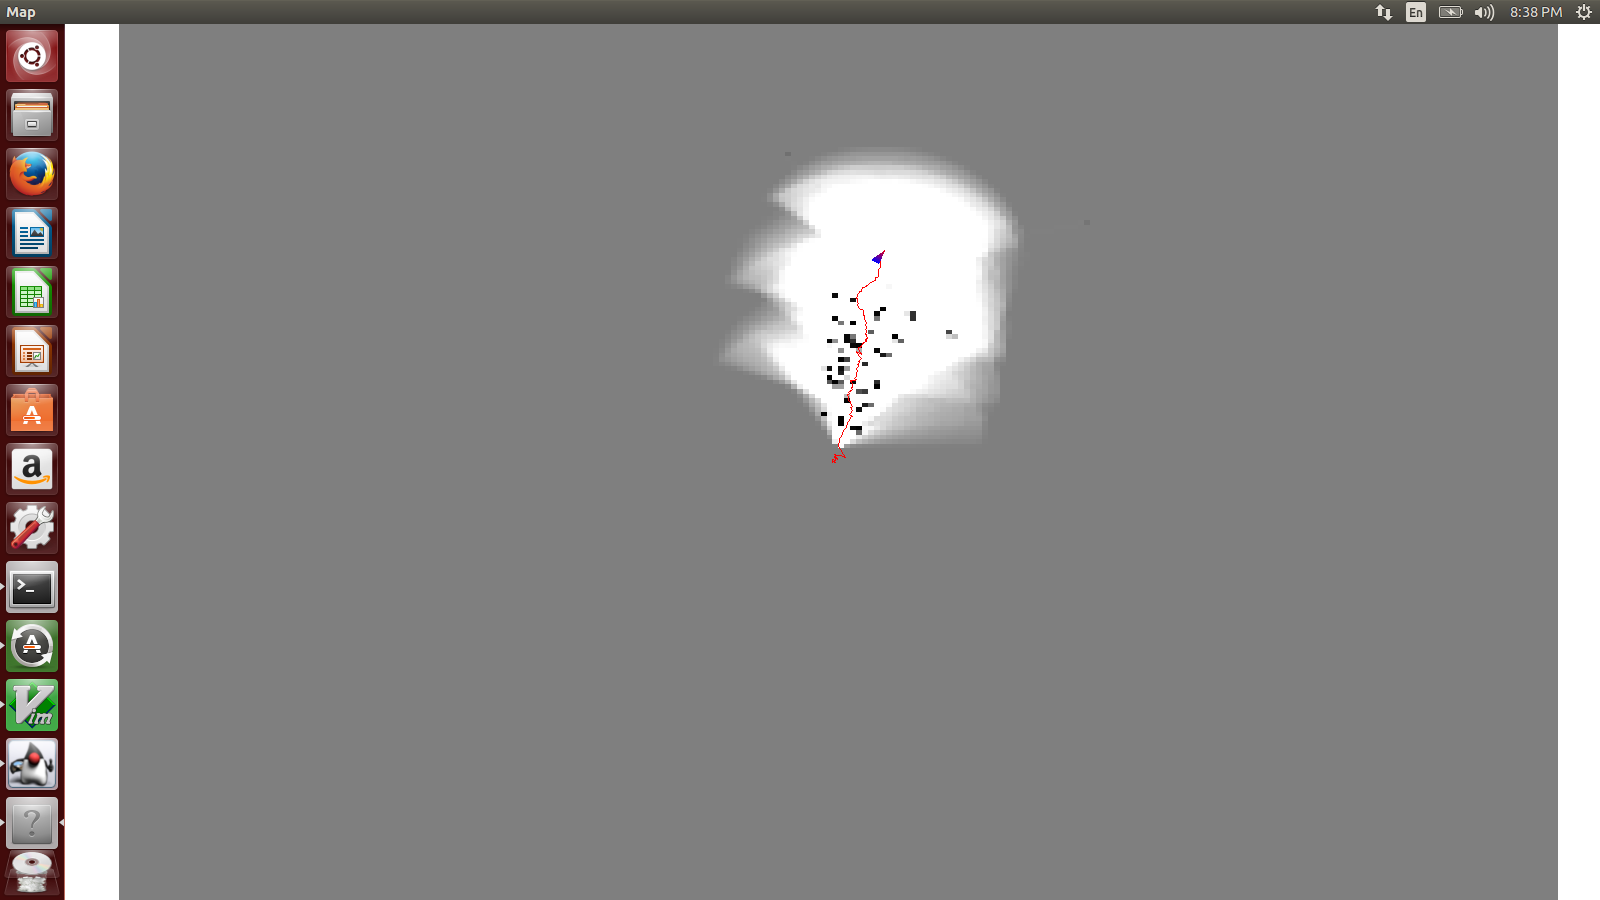
\includegraphics[trim={25cm 15cm 20cm 7cm}, clip, width=0.3\textwidth]{Figures/bigGrid}
	\caption{Maps generated using various grid sizes.  The left uses a grid cell size of 
	0.375 meters, the center is the baseline with a grid cell size of 0.5 meters,
	and the right is a grid cell size of 0.625 meters.}
	\label{fig:Grid Comparison}
\end{figure*}
The baseline performance of the system can be seen in Figure \ref{fig:Baseline}.  It
performed fairly well, but there are some problems that are still encountered when
you compare the camera feed in the log, to the map that is generated.
The first error that can be seen is the location of the objects.  The objects themselves
are about 15" in diameter, meaning that they should take up only a few cells, but some buoys
seem to drift over time and potentially merge with other buoys. In an ideal system, this
would not occur.  The other error that can be seen is close to the end of the ASV's path.
At the end, as it is exiting the buoy field, the ASV's pose is estimated to
be inside of a cell determined to be full.  Since the boat cannot occupy the same space as
a buoy, this is a misprediction.  

Overall, system performed quite well.  When comparing it to the camera
images in the log, the path closely matches the path the ASV appears to take through the
obstacle course, and the buoys appear to be in the same places the map  marks as full.
The combination of these factors makes the case that the SLAM system is performing fairly
well due to the accuracy of the results, but may have some issues with quasi static objects
such as buoys.

\subsection{Effects of varying grid cell size}
The size of grid cell has a fundamental effect on the performance of the SLAM system.
The primary effect occurs in the accuracy of the map.  By decreasing the cell size,
the map becomes more granular, causing objects to be potentially better defined.  However,
a more granular map can also cause issues with objects that are rather large, as more
data is needed to fill in the grid cells that it takes up.  Due to this, it is unknown
how a change in grid size will affect the map and paths generated.  
In addition to determining the granularity of the map, the size of the grid also affects
the runtime of the mapping process, since the number of squares a lidar scan goes through
is depedent on the size of a cell, as the cell size increases, the number of cells that
are updated decreases and vice versa.  This means that by increasing the granularity of the
map, the runtime also increases, an important consideration due to the goal of the system
running in real time.  

In this implementation, the grid size is determined by the constant \textbf{SQUARE\_SIZE},
seen in Appendix A, which represents the side length of a grid cell in meters. 
The baseline uses a value of 0.5, the small grid uses a value of 0.375, and the large
grid uses a value of 0.625.

To determine how the grid size affects the performance of the SLAM system the grid size
was varied over multpile runs and the maps produced with varying grid sizes can be seen
in Figure \ref{fig:Grid Comparison}.  In this Figure, the left most grid size was 0.375
meters per cell, the center is the baseline with 0.5 meters per cell, and the right most
grid size is 0.625 meters per cell.  For each of the cell sizes, the system was run
on the same log and every parameter other than the grid cell size remained the same value
as in the baseline.

When looking at the three grid sizes together, an interesting result is seen.  Both the
smaller and larger grids appear to merge objects together more than the baseline grid size
does.  For the larger grid size, this is an expected result.  For two objects close to each
other, it is more likely for the cells containing the two objects to be adjacent if the grid
cells are larger.  However, 
the merging is in contrast to what was expected for the smaller grid size.  By making the 
map more granular it is expected that object would not be merged together nearly as much, 
but would instead be more defined.  This unexpected merging may be caused by another effect
of lowering the grid cell size.  By lowering the grid cell size, while some objects became
smaller and more well defined, small errors in localization caused the location of objects
to jitter, and this jitter can drag objects along the path of the ASV.  This dragging
effect can be seen in the small grid size results in multple places.  By dragging the 
objects along with the ASV, the objects can be merged together, causing the merging
that was unexpected.

Of the three grid sizes tested, the baseline appears to create the best results, due to
the limited amount of merging that occurs.  Furthermore, due to the increase in runtime,
which was noticible, it is recommended to avoid decreasing the grid size if possible, due
to lack of improvment relative to the runtime costs.  Similarly due to the performance drop
that occurs when increasing the cell size, it is recommended that the cell size
is not increased due to the drop in mapping quality.

\subsection{Effects of varying number of particles}
Varying the number of particles changes the system in a few ways.  By increasing the amount
of particles, the number of possible poses increases, meaning that there is a better
likelihood of the correct pose being one of the particles.  The goal of varying the
number of particles is to see if increasing the particles increases the quality of the 
map and path produced, and to see if decreasing the number of particles causes a noticeable
decrease in the same numbers.
\begin{figure*}[t]
\centering
		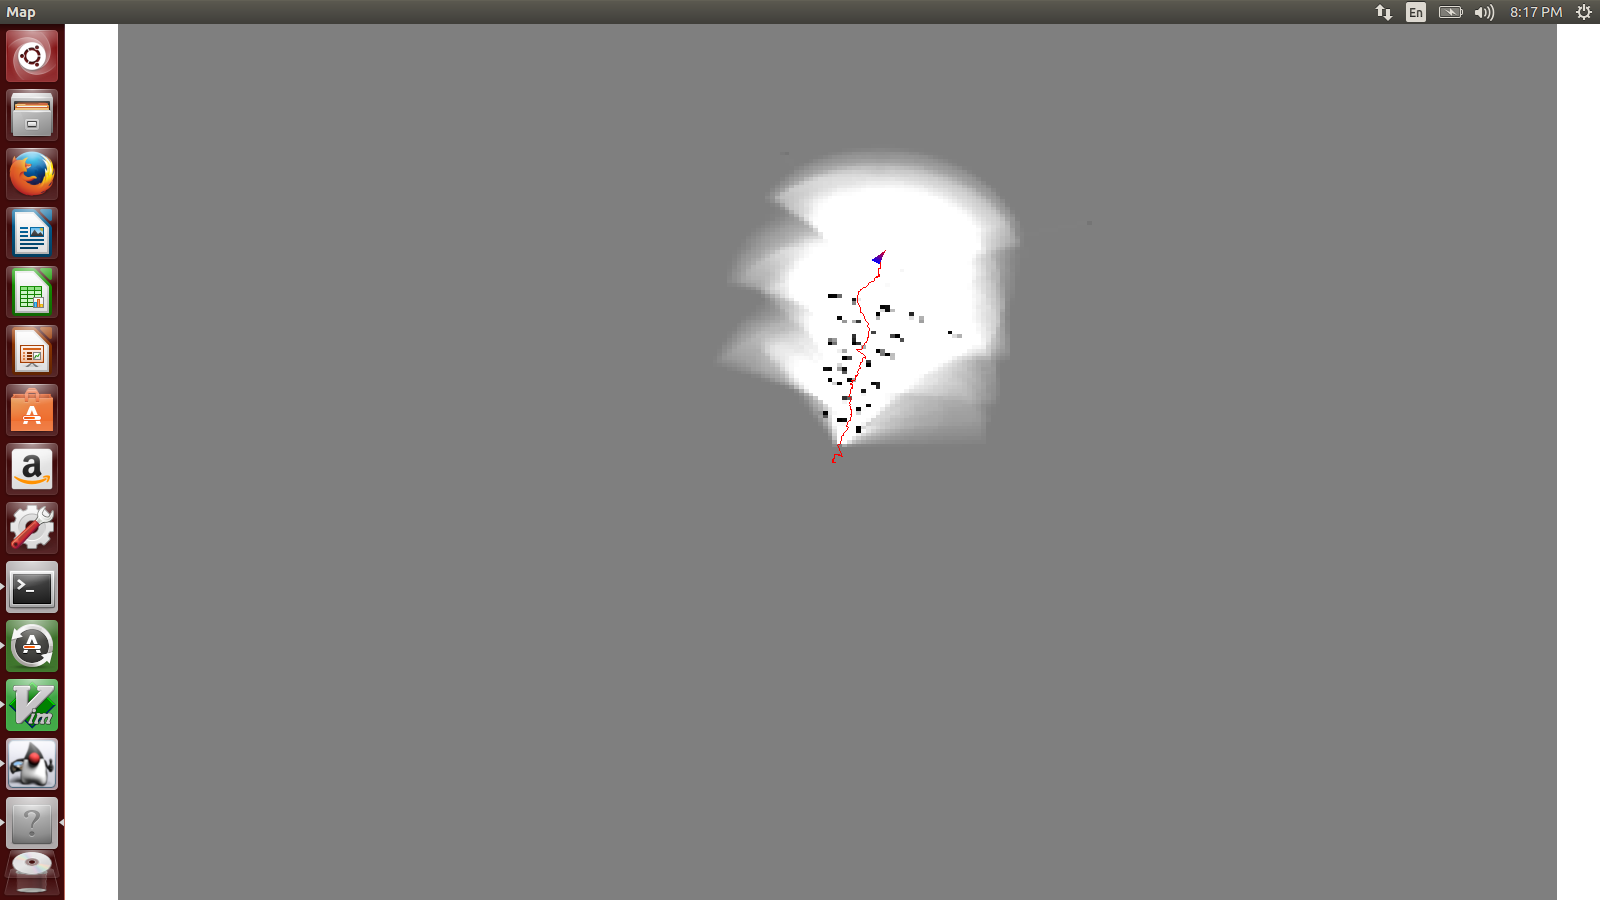
\includegraphics[trim={25cm 15cm 20cm 7cm}, clip, width=0.3\textwidth]{Figures/part500}
		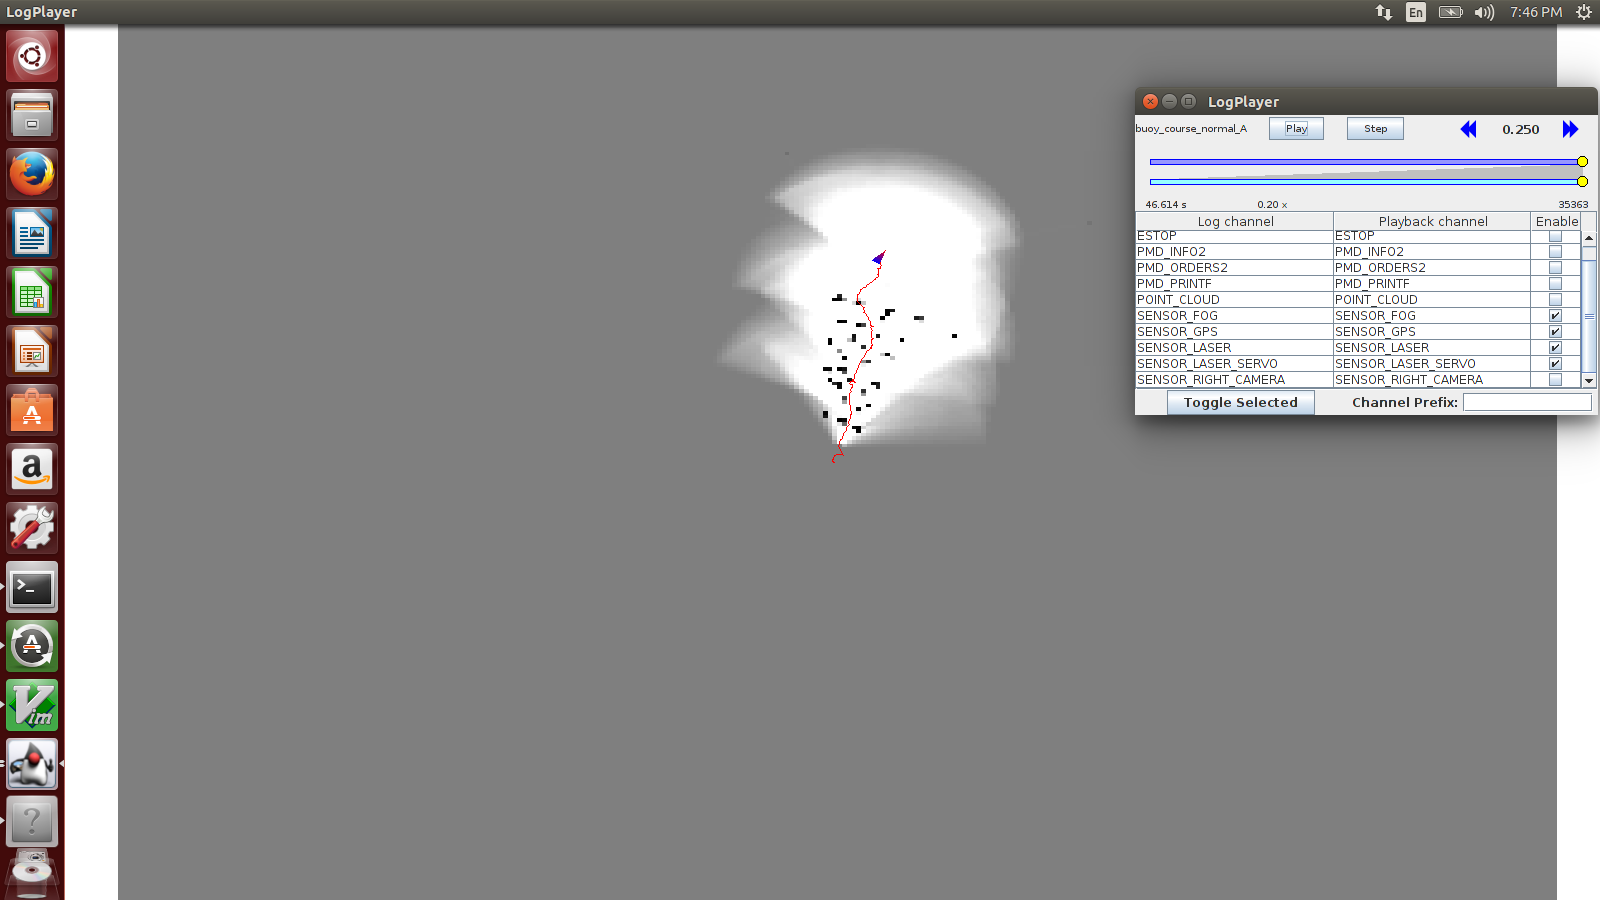
\includegraphics[trim={25cm 15cm 20cm 7cm}, clip, width=0.3\textwidth]{Figures/baseline1}
		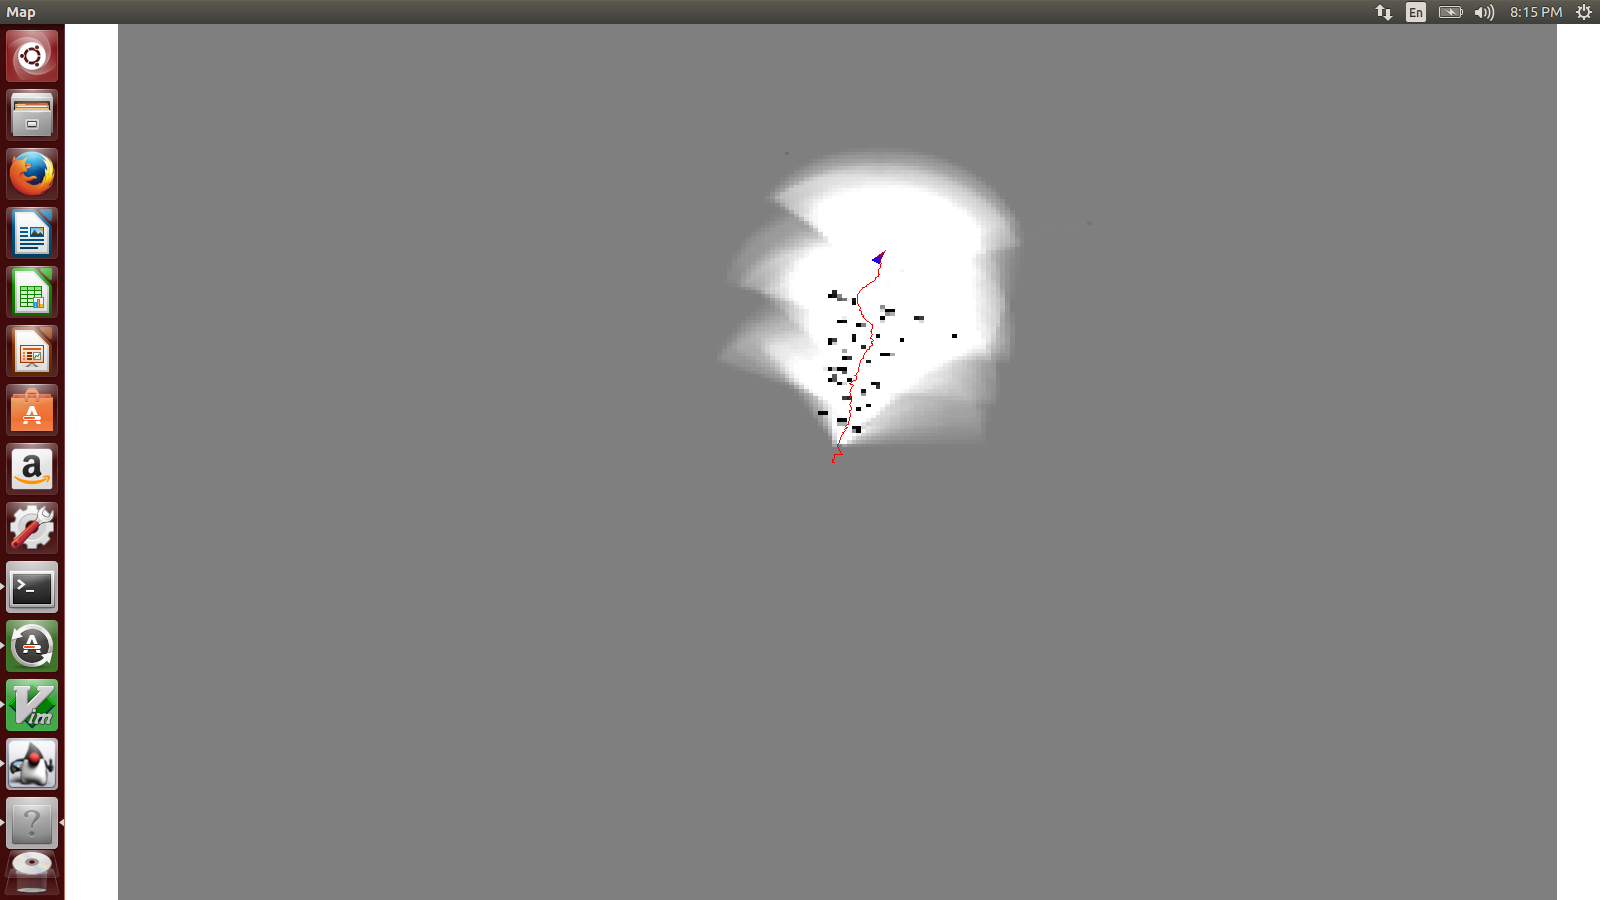
\includegraphics[trim={25cm 15cm 20cm 7cm}, clip, width=0.3\textwidth]{Figures/part2000}
	\caption{Comparison of varying the number of particles}
	\label{fig:Particle Comparison}
\end{figure*}

\begin{figure*}[t]
\centering
		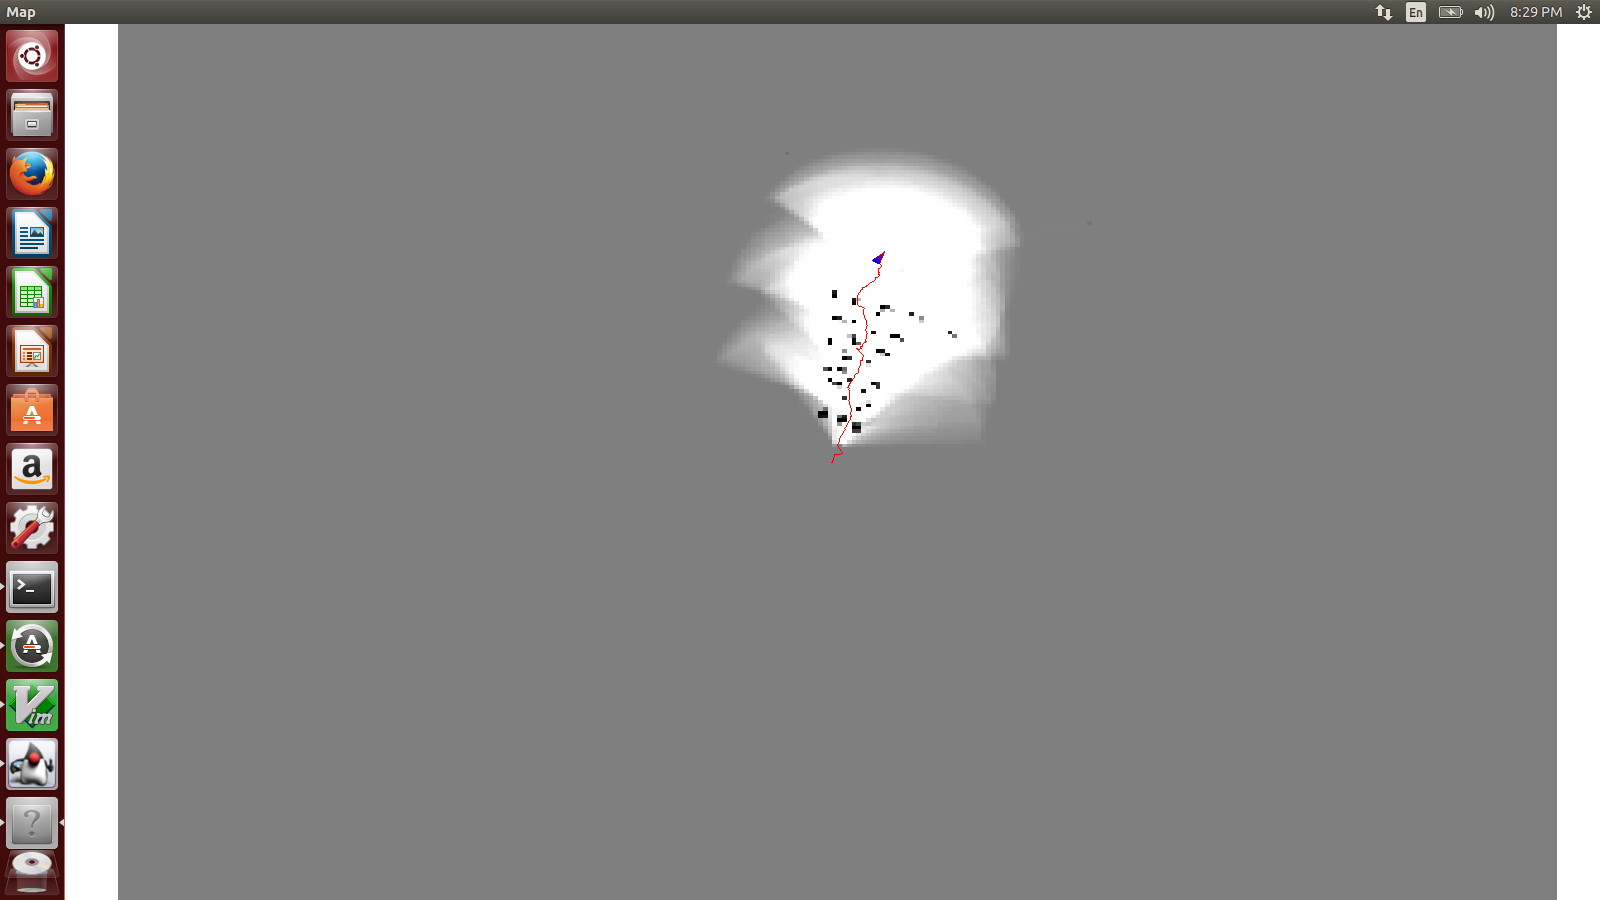
\includegraphics[trim={25cm 15cm 20cm 7cm}, clip, width=0.2\textwidth]{Figures/ratio0:1}
		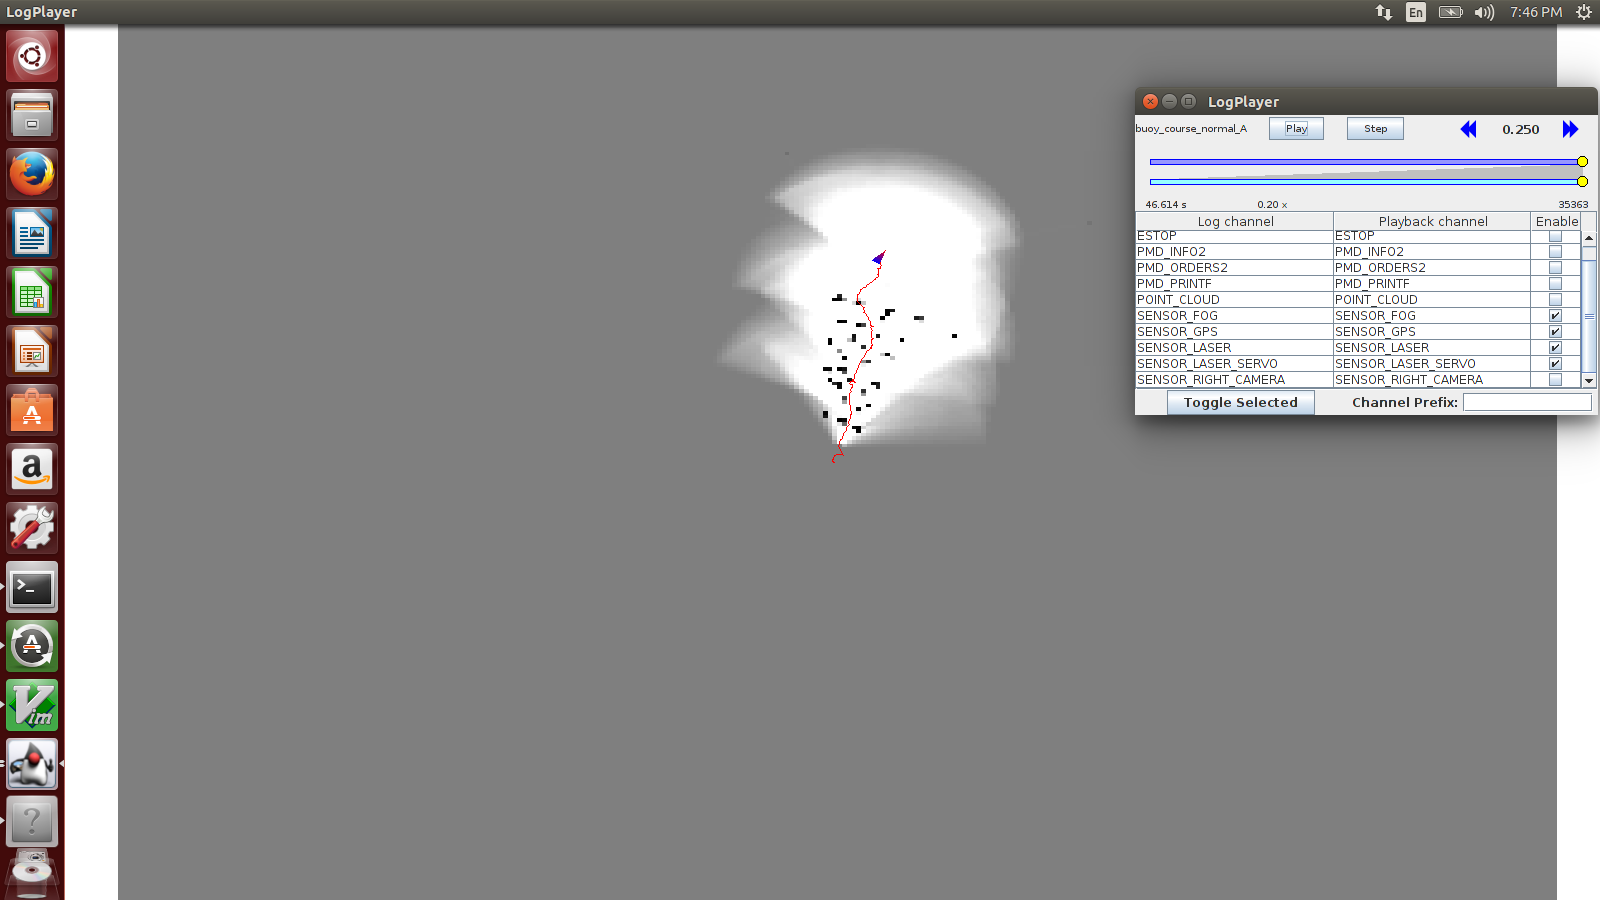
\includegraphics[trim={25cm 15cm 20cm 7cm}, clip, width=0.2\textwidth]{Figures/baseline1}
		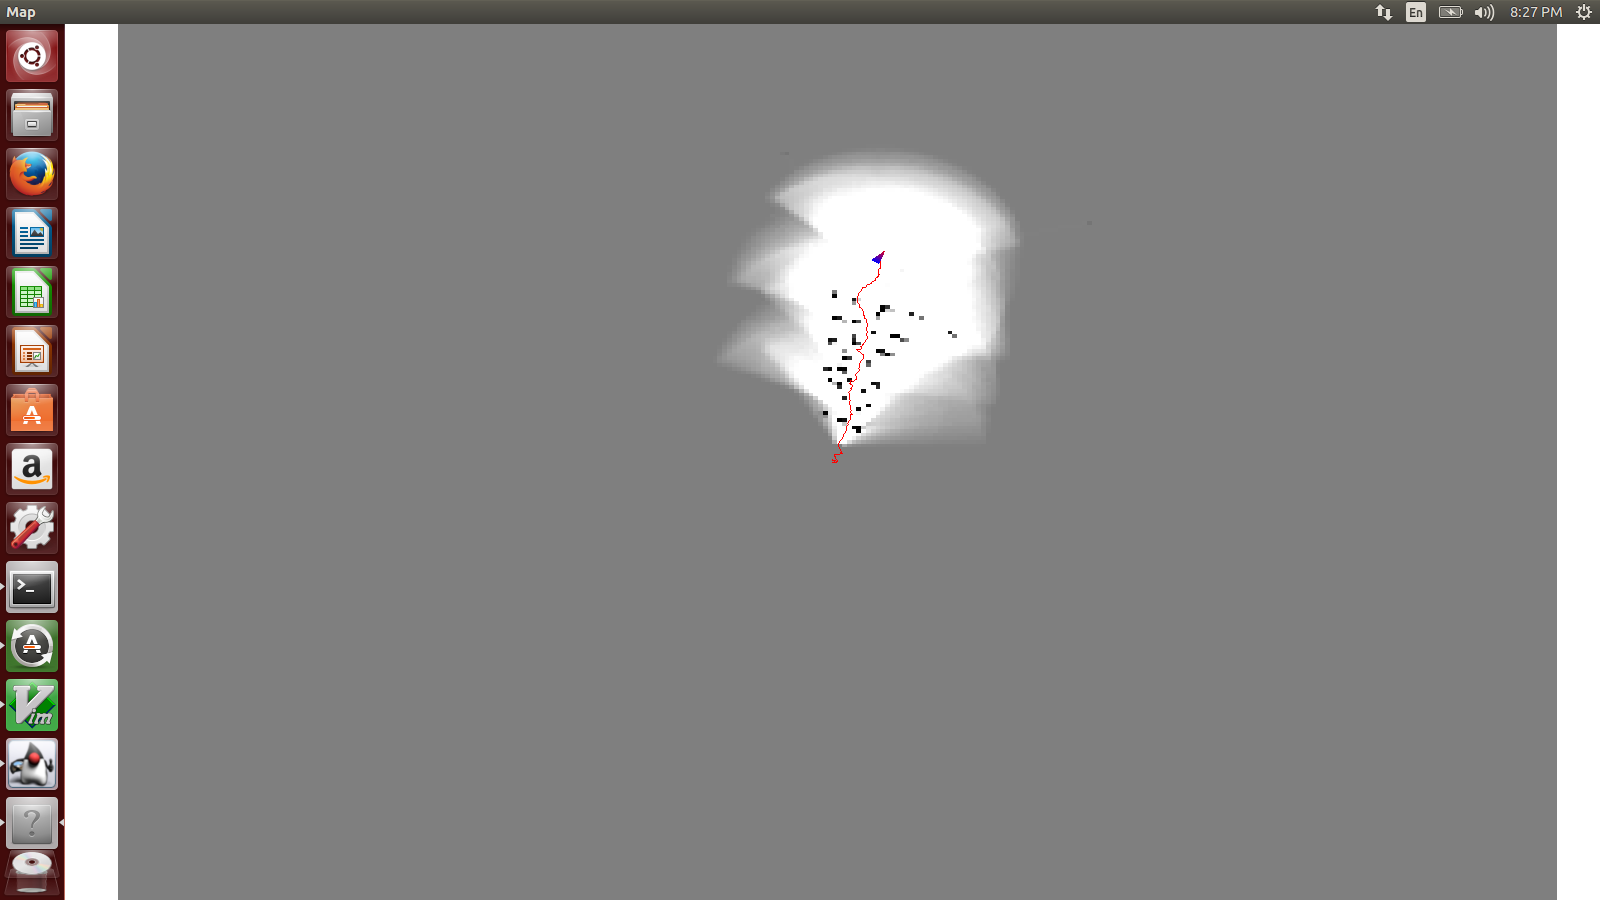
\includegraphics[trim={25cm 15cm 20cm 7cm}, clip, width=0.2\textwidth]{Figures/ratio1:1}
		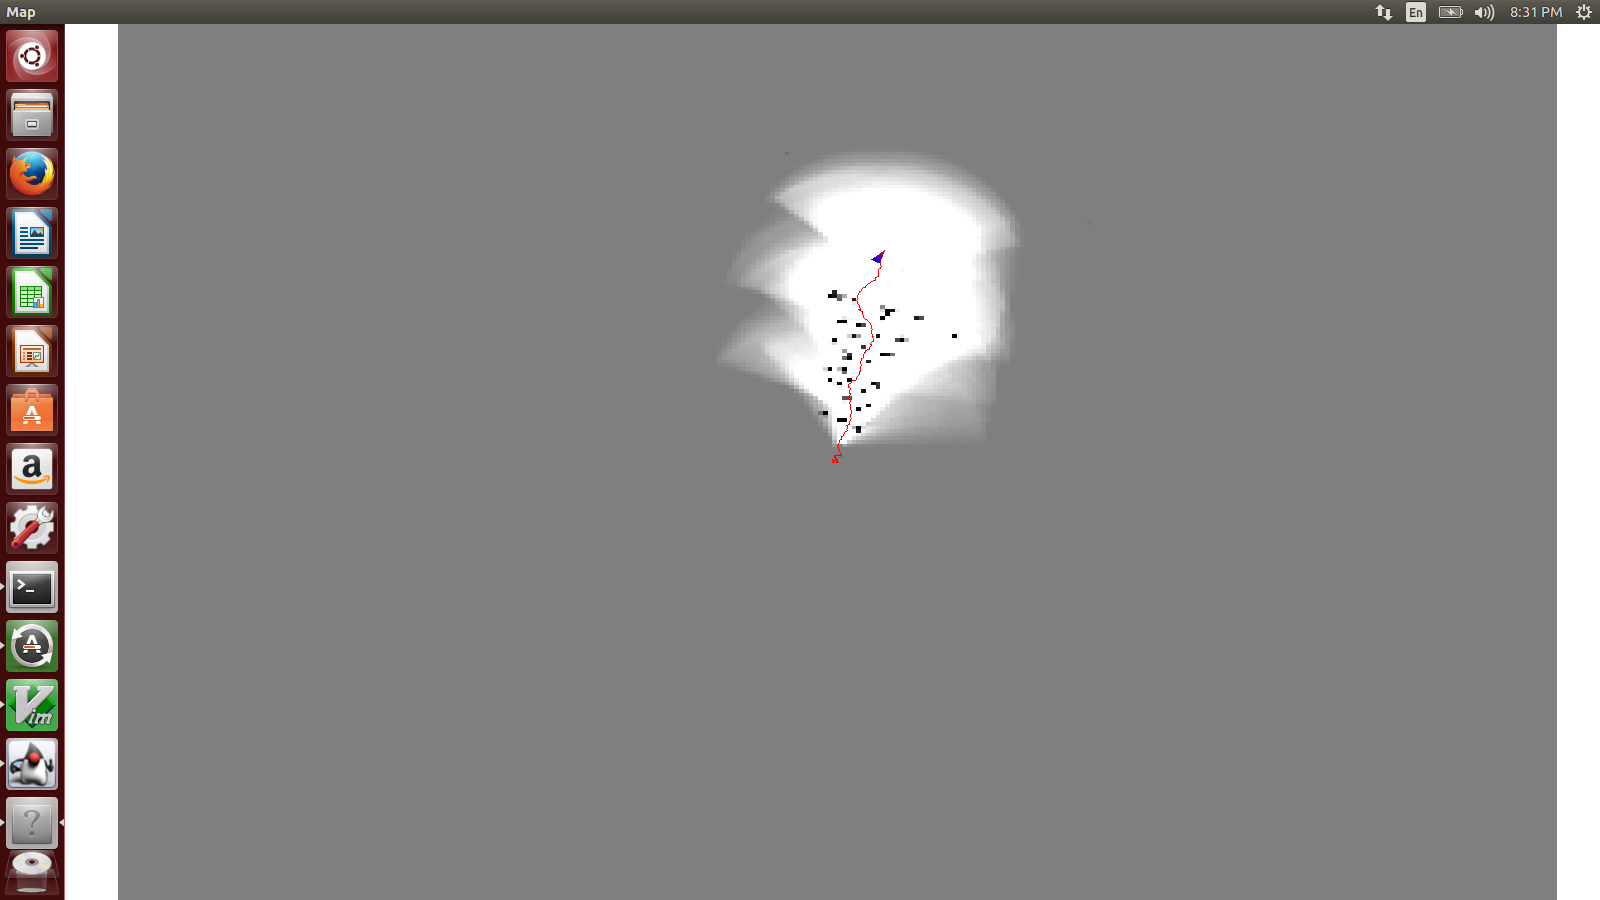
\includegraphics[trim={25cm 15cm 20cm 7cm}, clip, width=0.2\textwidth]{Figures/ratio1:0}
	\caption{Comparison of various ratios between lidar hit and lidar misses}
	\label{fig:Lidar Comparison}
\end{figure*}

This test was run in a way similar to the grid cell size tests.  All of the parameters 
remained the same between the baseline and the other tests besides the number of particles,
which is represented by the \textbf{NUM\_PARTICLES} constant in Appendix A.
The maps and predicted paths produced by the tests can be seen in Figure 
\ref{fig:Particle Comparison}.  The left most test used 500 particles per generation,
the baseline used
1000 particles each generation, and the right most test used 2000 particles for each 
generation.

When comparing the three tests, only a few differences can be seen.  This can mean
two things.  The first is that due to diminishing returns caused by a close enough particle
always being present, the number of particles may not significantly change the performance 
of the system.  The second possiblity is while this log may not show
significant differences, other logs may show differences.  These are two things that should
be investigated in future research.

In addition to these results, the number of particles also has an effect on runtime.  The 
implementation is such that the runtime of localization is linear in the number of particles,
so by doubling the number of particles, the runtime of localization is roughly
doubled.  When considering the benefits that may come with increasing the number of particles
it is important to always meet the runtime constraints.  The easiest way to decrease 
the runtime of the system is to decrease the number of particles. Since it appears
that the number of particles does not drastically affect the quality of the results, changing
the number of particles should be based on the desired runtime goals that need to be met.

\subsection{Effects of changing lidar hit and miss localization values}
This set of tests will vary the values that are used to generate the point cloud based
weights.  When referring to the hit reward, the value being talked about is the value added to a particle's point cloud based
weight when a lidar scan correctly ends in a space considered to be full, represented
by the constant \textbf{HIT\_LIKELIHOOD\_INC\_VALUE} in Appendix A.
Likewise when referring to miss penalty, the number being talked about
is the value by which a particle's point cloud based weight is decremented when a lidar 
return would end in a square considered to be empty, represented by the constant
\textbf{MISS\_LIKELIHOOD\_DEC\_VALUE} in Appendix A. 
The goal is to figure out what is the optimal 
ratio between rewarding correct lidar returns and penalizing incorrect lidar returns.
Based on the high accuracy of the lidar, it is expected that a miss penalty should be
greater than the hit reward.  

The results of this test can be seen in Figure \ref{fig:Lidar Comparison}.  The left most
test was run with only missed predictions being penalized.  The left middle is the baseline, run
with a ratio of 1:5 for hit rewards to miss penalties.  The right middle uses a ratio of 1:1,
and the right most only rewards correct predictions, and does not penalize misses.

The ratio of hit rewards to miss penalties does not appear to affect the quality of the
mapping process.   This is contrary to what was expected.  Instead, it appears that the 
weighting the points based on the number of incorrect predictions,
is similar in effect to weighting the particles based on correct predictions.  Upon
further analysis this makes sense.  A particle with more correct predictions consequentially
has less incorrect predictions and vice versa.  This leads to the conclusion that this
value does not necessarily need to be configurable due to its negligable effect.

\section{Conclusions}
In the end, the research has been successful in many areas.  Initially the research set out
to create a performant, useable, and maintainable SLAM system for an autonomous surface
vehicle. The initial analysis of the two possible solution methods showed that between 
iSAM and GM-MCL, in the long run the GM-MCL approach would most likely be more
maintainable than the iSAM solution, as well as more useable. Furthermore, due to the 
amount of acceptable error in the mapping process, the potentially better performance that
iSAM offers is negligable.

The GM-MCL based SLAM system developed in this project fits all the performance and 
useability goals.  It can run in real time, produces a reasonable map, and is useable by
someone without having an indepth knowledge of SLAM.  To increase maintainability of the
system, the code was written with readability and maintainability in mind.  Furthermore many
things were made to be configurable and those items are kept in a constants
file so that most changes only occur in one location.  This should lead to a system that
is maintainable within the context of the student team.


\bibliographystyle{IEEEtran}
\bibliography{IEEEabrv,SLAM_Report}

\newpage
\onecolumn
\appendix
\section{Baseline Constants File}
\begin{lstlisting}
#ifndef __SLAM_CONSTANTS_HPP__
#define __SLAM_CONSTANTS_HPP__

#include <cmath> //for M_PI

#define GPS_CHANNEL "SENSOR_GPS"
#define FOG_CHANNEL "SENSOR_FOG"
#define LASER_SCAN_CHANNEL "SENSOR_LASER"
#define STATE_CHANNEL "STATE_CHANNEL"
#define SERVO_CHANNEL "SENSOR_LASER_SERVO"
#define SLAM_STATE_CHANNEL "SLAM_STATE"
#define SLAM_POINT_CLOUD_CHANNEL "SLAM_POINT_CLOUD"
#define SLAM_PARTICLE_CHANNEL "SLAM_PARTICLES"

//profiling constants
#define NUM_PROFILED_SCANS 30

//general constants (FULL SLAM)
#define NUM_ONLY_MAP_SCANS 1
#define MAX_X 75
#define MIN_X -75
#define MAX_Y 75
#define MIN_Y -75
#define SQUARE_SIZE 0.5

//localization constants
const static int HIT_THRESHOLD = 160;
const static int MISS_THRESHOLD = 75;
const static int NUM_AVERAGE_PARTICLES = 1;
const static int NUM_OUTLIERS_TO_REMOVE = 0;
const static int NUM_PARTICLES = 1000;

//Lidar related localization coefficients
const static double HIT_LIKELIHOOD_INC_VALUE = 1.0;
const static double MISS_LIKELIHOOD_DEC_VALUE = -5.0;
const static int MINIMUM_LIDAR_HITS_TO_WEIGHT = 100;

//GPS related localization coefficients
//unit is meters
//Data sheet values 1.5
const static double DEFAULT_GPS_SIGMA = 1.5;

//FOG related localization coefficients
//unit is radians
//Data sheet value 0.5
const static double DEFAULT_FOG_SIGMA = 0.5*M_PI/180.0;

//Localization coefficients related to predicting particles forward with gps
const static double PERCENT_PREDICTION_PARTICLES = 0.50;
const static double X_PREDICTION_SIGMA = 0.1;
const static double Y_PREDICTION_SIGMA = 0.1;

//Localization constants that relate the relative beliefs in the various sensors
const static double LASER_LIKELIHOOD_COEFFICIENT = 0.75;
const static double GPS_LIKELIHOOD_COEFFICIENT = 2.5;
const static double FOG_LIKELIHOOD_COEFFICIENT = 1.0;

//mapping constants
#define INITIAL_MAP_VALUE 128
#define FULL_SQUARE_INC 5.0
static const double EMPTY_SQUARE_INC = -0.025;
static const double LIDAR_MAP_RANGE_DEG = 60.0;

//point cloud constants
#define DEFAULT_MISS_RANGE 15
static const double LIDAR_HEIGHT = 0.15;

//fake compass stuff
#define USE_FAKE_COMPASS 1
#define ORIGIN_DIST_BEFORE_REINITIALIZATION 5

//Drawing stuff
#define NUM_POSES_TO_DRAW 50

#endif
\end{lstlisting}

\end{document}
